%%Sorting Networks File. 

%Intro subsection
\section{Sorting Networks}
\subsection{Introduction}
Let a \emph{wire} be a horizontal line. Let a \emph{comparator} be a vertical line connecting two wires. A 
\emph{sorting network} is a device consisting of $[1 \dots N]$ wires and $[0 \dots M]$  
comparators such that the sorting network sorts a permutation of $N$ elements into ascending order. The 
$N$ elements are first listed to the left of each wire in the network. The elements travel across their respective wires 
at the same time. When a pair of elements, traveling through a pair of wires, 
encounter a comparator, the comparator swaps the elements if and only if the top wire's element 
is greater than the bottom wire's element. A sorting network with $N$ wires and $M$ 
comparators that can sort any permutation of order $N$ is a \emph{complete sorting network}. 
To see a complete sorting network for $N=4$ please refer to Fig.\ref{Fig:SortNetwork}. \par 

\begin{figure}
    \centering
    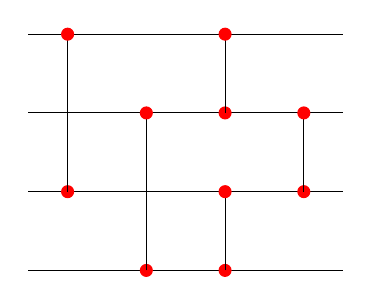
\begin{tikzpicture}
        \draw(0, 0) to (4, 0);
           
        \draw(0, 1) to (4, 1);
        \draw(0, 2) to (4, 2);
           
        \draw(0, 3) to (4, 3);

        %%connector 1
        \draw[red, fill=red](.5,1) circle (.5ex);
            \draw(.5, 1) to (.5, 3);
        \draw[red, fill=red](.5,3) circle (.5ex);


        %%connector 2 
        \draw[red, fill=red](1.5,0) circle (.5ex);
            \draw(1.5, 0) to (1.5, 2);
        \draw[red, fill=red](1.5,2) circle (.5ex);

        %%connector 3
        \draw[red, fill=red](2.5,2) circle (.5ex);
            \draw(2.5, 2) to (2.5, 3);
        \draw[red, fill=red](2.5,3) circle (.5ex);

        \draw[red, fill=red](2.5,0) circle (.5ex);
            \draw(2.5, 0) to (2.5, 1);
        \draw[red, fill=red](2.5,1) circle (.5ex);
        
        %%connector 4
        \draw[red, fill=red](3.5,1) circle (.5ex);
            \draw(3.5, 1) to (3.5, 2);
        \draw[red, fill=red](3.5,2) circle (.5ex);


    \end{tikzpicture}
    \caption{Complete Sorting Network for $N=4$.}
    \label{Fig:SortNetwork}
\end{figure}

Sorting networks were first studied in 1954 by Armstrong, Nelson and O'Connor. 
Sorting networks can be implemented either in hardware or in software \cite{A18}.
Donald Knuth describes how the comparators for binary integers can be implemented as simple, 
three-state electronic devices \cite{A18}. Batcher, in 1968, 
suggested using them to construct switching networks for computer hardware, replacing 
both buses and the faster, but more expensive, crossbar switches \cite{A27}. Since the 2000s, sorting networks are used by the 
\emph{general purpose graphics processing unit community}, which are a group of people who use 
the GPU for non-graphical programming, for constructing sorting algorithms \cite{A28}.\par 
Sorting networks are intricately related to ladder-lotteries. Let a \emph{minimum sorting network} be defined 
as a sorting network such that for any arbitrary comparator, $c$, on wire $i$, $c$ connects to line $i+1$ or $i-1$. Furthermore, 
the number of comparators in a minimum sorting network is equal to the number of inversions in $\pi$. Clearly there is a 
one to one mapping from the comparators in a minimum sorting network to the bars in an optimal ladder lottery and there 
is a one to one mapping from the wires in a minimum sorting network and the lines in a ladder lottery \cite{A29}. 


 
\subsection{The Integer Sequence Relating to the Reverse Permutation}
Let $Rev(\pi)$ refer to the reverse permutation of $[1 \dots N]$. There is an integer sequence that counts the number of minimum sorting networks 
for $Rev(\pi$). This integer sequence also counts $OptL\{Rev(\pi)\}$. This sequence grows very quickly, therefore $N=15$ 
is  the largest value this integer sequence has been calculated for. To refer to the table for this sequence 
please refer to Table \ref{Tab:IntSeq1} \cite{A30}.
There is currently no known closed form solution for this sequence. 
Thus, new values of $N$ are counted by a variety of algorithms. 
In their paper, \textbf{Efficient Enumeration of all Ladder Lotteries and its Application}, 
the authors were the first to calculate the sequence for $N=11$ \cite{A1} with the algorithm $FindAllChildren$ \ref{Alg:FindAllChildren}. 
In the paper \textbf{Counting Primitive Sorting Networks by $\mathbb{\pi}$DDs}, the authors were the first to caluclate for 
$N=13$ with a data structure they have termed $\mathbb{\pi}$DD \cite{A29}. The data structure is a digraph that holds a 
set of elementary permutations along with a number of operations that are applied to the elemetary permutations \cite{A29}.
The data structure resembles a digraph with two sink node; one sink node is labelled the zero sink node and the other 
is labelled the one sink node \cite{A29}. A $\mathbb{\pi}$DD is defined as follows \cite{A29}: 
\begin{itemize}
    \item There are two sink vertices labelled the zero and one sink node.
    \item Each other vertex has two outgoing edges labelled with a zero or one known as the \emph{zero edge} and \emph{one edge} respectively
    \item Each vertex $P$ is labelled by a tuple $(xP$,$yP) \in S X S$ where $S$ is an elementary permutation and $xP > yP$. 
    \item  (ordered) If the 0-edge of a vertex P points Q, then either $xP = xQ$ and
            $yP < yQ$ or $xP > xQ$ holds. If the 1-edge of a vertex P points R, then
            $xP > xR$ holds.
    \item There is no vertex P whose 1-edge directly points the 0-terminal
    \item There are no distinct vertices P and Q such that
        – $(xP, yP) = (xQ, yQ)$\newline
        – their 0-edges point the same vertex\newline
        – their 1-edges point the same vertex\newline
\end{itemize}

Each vertex P represents a set $\Pi P$ of permutations. Let $\tau xP, yP$ be defined as a transposition 
of $x,y \in P$. $P$ is recursively defined as follows:
\begin{itemize}
    \item if $P$ is the zero sink then $P=\emptyset$
    \item else if $P$ is the one sink then  $P=\pi_{ID}$
    \item else $\Pi P = \Pi Q \cup (\Pi R . \tau xP,yP)= \Pi Q \cup \{\pi \tau xP, yP | \pi \in R\}$ whose $0$ egde points to $Q$ and whose $1$ edge points to $R$.
\end{itemize}
\pagebreak



\begin{table}
    \begin{center}

    \begin{tabular}{|p{2cm}||p{8cm}|}
        \hline
        \multicolumn{2}{|c|}{Number of minimum sorting networks/$|OptL\{Rev(\pi)\}|$}\\
        \hline
        N & Count \\ 
        \hline 
        1 & 1 \\
        \hline 
        2 & 1 \\
        \hline 
        3 & 2 \\
        \hline 
        4 & 8 \\
        \hline 
        5 & 62 \\
        \hline 
        6 & 908 \\
        \hline 
        7 & 24698 \\
        \hline 
        8 & 1232944 \\
        \hline 
        9 & 112018190 \\
        \hline 
        10 & 18410581880 \\
        \hline 
        11 & 5449192389984 \\ 
        \hline 
        12 & 2894710651370536 \\
        \hline 
        13 & 2752596959306389652 \\
        \hline 
        14 & 4675651520558571537540 \\
        \hline 
        15 & 14163808995580022218786390 \\
        \hline 
    \end{tabular}
    \end{center}
    \caption{Number of minimum sorting networks and $|OptL\{Rev(\pi)\}|$}
    \label{Tab:IntSeq1}
\end{table}\par